\subsection{Cyber-Physical Systems and Hybrid Dynamical Systems}

\textbf{Cyber-Physical System (CPS):} the systems combine 
\ctextbf{cyber capabilities} with \ctextbf{physical capabilities} 
to solve problems that \ctextit{neither part could solve alone}.

From a mathematical perspective, cyber-physical systems are ($\subseteq$) 
\ctextbf{Hybrid Dynamical Systems}:

\textbf{Hybrid Dynamical System (HDS):} the systems are a mathematical model 
of dynamical systems that 
\ctextit{combine discrete dynamics with continuous dynamics}.
Their behavior includes both  
\vspace{-.5cm}
\begin{itemize}
  \item aspects that \ctextit{change discretely one step at a time}, and
  \item aspects that \ctextit{change continuously as continuous 
    functions over time}.
\end{itemize}

In the most naive interpretation, 
\vspace{-.5cm}
\begin{itemize}
  \item $\text{cyber components of CPSs} \xrightarrow[\text{correspond to}]
    {directly} \text{discrete dynamics of HDSs}$,
  \item $\text{physical components of CPSs} \xrightarrow[\text{correspond to}]
    {directly} \text{continuous dynamics of HDSs}$.
\end{itemize}

However, there are events in physical models that are best described by 
a discrete dynamics even if they come from the physics, and vice versa.
For example, 
\vspace{-.5cm}
\begin{itemize}
  \item The touchdown of an airplane on the ground 
    ($\text{Physical component} \to \text{Discrete dynamics}$),
  \item The PID controller 
    ($\text{Cyber component} \to \text{Continuous dynamics}$).
\end{itemize}

By the way, a number of cyber-physical systems feature additional 
  aspects beyond hybrid systems,
such as \ctextbf{adversarial dynamics}, \ctextbf{distributed dynamics},
  or \ctextbf{stochastic dynamics}.

\subsubsection{Multi-dynamical Systems}

CPSs are treated as a \ctextit{combination of multiple elementary} 
dynamical aspects.
The key to this mystery is to integrate the CPS dynamics all within a single,
\ctextbf{Compositional Logic}.

\textbf{Multi-dynamical system:} the systems are mathematical models of 
dynamical systems characterized by multiple facets of dynamical systems, 
schematically includes:
\vspace{-.5cm}
\begin{itemize}
  \item Part A: discrete $\cap$ continuous;
  \item Part B: adversarial $\cap$ non-deterministic $\cap$ stochastic.
\end{itemize}


\subsubsection{Methodology}

Dependencies and suggested reading sequences of the chapters are presented in 
Fig. \ref{fig:socps}.

\begin{figure}[H]
  \centering
  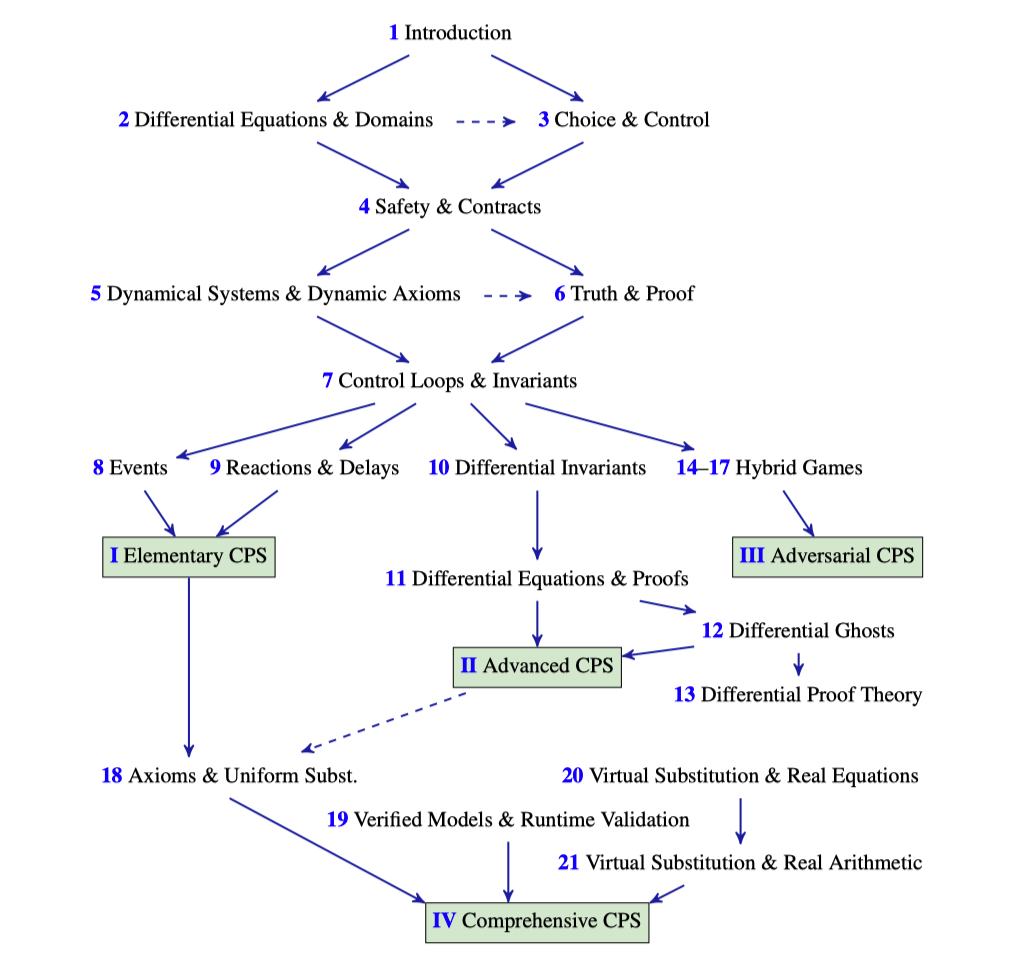
\includegraphics[width=.85\linewidth]
    {notes/hybrid-dynamical-system/figures/structure-of-cps.png}
  \caption{Dependencies and suggested reading sequences}
  \label{fig:socps}
\end{figure}

\crule